
\documentclass[10pt,a4paper]{article}
\usepackage[utf8]{inputenc}
\usepackage[spanish]{babel}
\usepackage{amsmath}
\usepackage{amsfonts}
\usepackage{amssymb}
\usepackage{makeidx}
\usepackage{graphicx}
\usepackage{cite} % para contraer referencias
\usepackage{fourier}
\usepackage{xcolor}
\usepackage{hyperref}
 \usepackage{float}
\usepackage[bottom]{footmisc}
\usepackage[left=2cm,right=2cm,top=2cm,bottom=2cm]{geometry}
\title{Plan - sesión 4}


\author{\textbf{Victor M. Santos}\thanks{victorhugo\_m09@hotmail.com}, \textbf{M.Tarazona-Alvarado}\thanks{miguelta281@gmail.com}, \textbf{J. Pisco-Guabave} \thanks{jhojavi@gmail.com}. \\ Grupo Halley , \\ Universidad Industrial de Santander, Bucaramanga, Colombia.}


\date{ }


\begin{document}

\maketitle
\tableofcontents
\section{Objetivo}
Conocer las constelaciones junto con la carta celeste y algunas aplicaciones que facilitan la observación celeste.

\section{Contenido}
\begin{itemize}
\item Constelaciones
\item Carta celeste
\item Aplicaciones usadas en la astronomía
\end{itemize}


\section{Recursos}
\begin{itemize}
 \item Salón con capacidad para 20 personas
 \item Proyector
 \item Computador
 \item Marcadores
 \item Tablero
 \item Espacio al aire libre (amplio)
\end{itemize}

\section{Marco conceptual}

\subsection{Constelaciones oficiales}
Una constelación es una agrupación convencional de estrellas cuya posición en el cielo nocturno es aparentemente invariable.\\

Generalmente, las civilizaciones antiguas creaban siluetas  imaginarias sobre la esfera celeste. Distintas culturas han ideado constelaciones diferentes, incluso vinculando las mismas estrellas. Existen dos grandes clasificaciones en las constelaciones:

\begin{itemize}
    \item Constelaciones septentrionales (hemisferio norte).
    \item Constelaciones australes (hemisferio sur).
\end{itemize}

A partir de 1928, la Unión Astronómica Internacional (IAU) decidió agrupar oficialmente la esfera celeste en 88 constelaciones con límites precisos. 

\subsubsection{Constelaciones Zodiacales}

\begin{itemize}
 \item \textbf{Aries:} también conocida como el carnero, había sido enviada por Zeus para rescatar a dos niños de sus madrastra, era un borrego volador. Después de muerto, su piel de oro se convirtió en un tesoro codiciado por Jason y los argonautas, quienes se metieron en muchos aprietos para robarla.
 
\begin{figure}[H]
\centering
%\raggedright
\includegraphics[scale=0.18]{Imagenes/Aries_01}
\end{figure} 

 \item \textbf{Taurus:} Zeus se disfrazó de un toro llamado Taurus, de esta forma se acercó cariñosamente a una princesa muy hermosa llamada Europa; acostada en el lomo de Taurus huyeron cruzando el mar hasta la isla de Creta. Ahí, Zeus reveló su identidad y la pareja fue feliz... hasta que Zeus conoció a Leda.
 
\begin{figure}[H]
\centering
%\raggedright
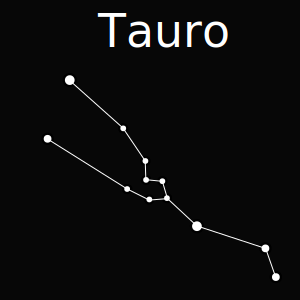
\includegraphics[scale=0.18]{Imagenes/Tauro_01}
\end{figure} 

 \item \textbf{Gemeni:} Zeus se disfrazo de Cygnus, el cisne, para enamorar a Leda y tuvieron dos hijos que llamaron Castor y Póllux. Estos dos también se unieron en la búsqueda de la piel dorada de Aries, pero Castor murió y Póllux se puso muy triste. Entonces, Zeus decidió unirlos en el cielo y ahora forman la constelación de Gemini.
 
\begin{figure}[H]
\centering
%\raggedright
\includegraphics[scale=0.18]{Imagenes/Geminis_01}
\end{figure}  
 
 \item \textbf{Cancer:} una vez el poderoso Hércules se enfrentó con Hidra, una serpiente enorme de nueve cabezas. Juno, que era enemiga de Hércules, le complico la pelea enviándole un cangrejo que le pellizcara los talones. Hércules lo vio y lo aplastó de un pisotón. La obediencia del cangrejo fue recompensada por Juno, que puso al cangrejo entre las constelaciones.
 
\begin{figure}[H]
\centering
%\raggedright
\includegraphics[scale=0.18]{Imagenes/Cancer_01}
\end{figure}   
 
 \item \textbf{Leo:} en una pelea, Hércules se enfrentaba contra un extraterrestre: un león que había llegado de la Luna. Hércules estrangulo al gran felino, colgando su piel como una capa sobre su espalda a modo de trofeo.

\begin{figure}[H]
\centering
%\raggedright
\includegraphics[scale=0.18]{Imagenes/Leo_01}
\end{figure}  

 \item \textbf{Virgo:} en muchas culturas se veían vírgenes entre los personajes del cielo. Entre ellas Virgo, quien representa a Ceres, la diosa de las cosechas.
 
\begin{figure}[H]
\centering
%\raggedright
\includegraphics[scale=0.18]{Imagenes/Virgo_01}
\end{figure}   
 
 \item  \textbf{Libra:} otra dama mitológica es Astrea, diosa romana de la justicia, los hombres la recordaban cuando veían la constelación de Libra, la balanza que ella mostraba en alto y que representaba su equidad.

\begin{figure}[H]
\centering
%\raggedright
\includegraphics[scale=0.18]{Imagenes/Libra_01}
\end{figure}  

 \item \textbf{Scorpius:} en otro tiempo, las estrellas de Libra dibujaban las tenazas de un arácnido, un escorpión llamado Scorpius. Por órdenes de Apolo, el escorpión atacó a Orión, todo porque Orión pretendía a Artemisa\footnote{Diosa de la Luna y hermana de Apolo.}. Desde entonces, escorpius persigue a Orión para matarlo.
 
\begin{figure}[H]
\centering
%\raggedright
\includegraphics[scale=0.18]{Imagenes/Escorpio_01}
\end{figure} 
 
 \item \textbf{Sagitarius:} los dioses tenían habilidades muy preciadas, por ejemplo el arquero Sagitarius, Quiron. Era un centauro famoso por su talento como músico y médico, quien también era un gran arquero pero no lo aceptaron los humanos por ser un centauro.
 
 \begin{figure}[H]
\centering
%\raggedright
\includegraphics[scale=0.18]{Imagenes/Sagitario_01}
\end{figure} 
 
 \item \textbf{Capricornus:} por andarse metiendo donde no debía, Pan fue perseguido por Tifón, un monstruo. Para escapar del monstruo, el semi-dios se arrojó al río Nilo, pero sus manos y cabeza, aún fuera del agua, se transformaron en cabra; mientras las partes que estaban sumergidas se convertían en pez. Ahora se le conoce como Capricornus, la cabra marina.
 
 \begin{figure}[H]
\centering
%\raggedright
\includegraphics[scale=0.18]{Imagenes/Capricornio_01}
\end{figure}

 \item \textbf{Aquarius:} una leyenda cuenta que la temporada de lluvia es culpa de Aquarius. Es un muchacho que pasa corriendo por el cielo y en sus manos lleva un canto lleno de agua, agua que es derramada por distracción de Aquarius.
 
 \begin{figure}[H]
\centering
%\raggedright
\includegraphics[scale=0.18]{Imagenes/Acuario_01}
\end{figure} 
 
 \item \textbf{Piscis:} Venus y Cupido también fueron perseguidos por Tifón y para escapar se arrojaron al río Éufrates, donde se convirtieron en peces y nadaron a un lugar seguro. Hoy vemos a Venus y Cupido unidos por un largo cordón en la constelación de Piscis.
 
  \begin{figure}[H]
\centering
%\raggedright
\includegraphics[scale=0.18]{Imagenes/Pisis_01}
\end{figure}
\end{itemize}

\subsubsection{Constelaciones septentrionales}
\begin{itemize}
 \item \textbf{Dragón:} \textit{Thuban}\footnote{La cola del dragón.} fue la \textit{Polar} hace 4500 años, debido a la precesión de los equinoccios se ha desplazado cediendo el lugar de \textit{Polar} a \textit{Polaris}\footnote{Actual estrella polar.}. La constelación del \textit{Dragón} es una constelación grande y de poco brillo que envuelve a la \textit{Osa Menor}. Contiene una nébulasa planetaria.
 
 \item \textbf{Cefeo:} representa al legendario rey de \textit{Etiopía}, esposo de \textit{Casiopea} y padre de \textit{Andrómeda}. La constelación de \textit{Cefeo} tiene forma de casa con un techo en punta.

 \item \textbf{Casiopea:} con forma de ``M" cruzada sobre la vía láctea. Madre de \textit{Andrómeda}. Cuenta la historia que \textit{Casiopea} alardeaba de su belleza, comparándola con la de las \textit{Nereidas}\footnote{Hijas de \textit{Nereo} y \textit{Doris}.}, hijas del dios del mar y conocidas como las criaturas más bellas de todas. \textit{Casiopea} señala el norte con sus extremos.
 
 \item \textbf{Pegaso:} es un cuadrilátero, comparte estrella con Andrómeda. Era un caballo alado, específicamente el caballo de Zeus. Nació de la mezcla de espuma de mar con la sangre que brotó de la cabeza de cabeza de Medusa cuando Perseo la cortó.
 
 \item \textbf{Andrómeda:} se sitúa al sur de Casiopea y cerca a Pegaso, además comparte una estrella con Pegaso. Andrómeda es hija de Cefeo y Casiopea, y también esposa de Perseo.
 
 \item \textbf{Fenix:} narra la historia de un ave capaz de renacer de sus propias cenizas. Representa la delicadeza, ya que vive solo del rocío y sin lastimar a ninguna otra criatura viviente.
 
 \item \textbf{Perseo:} en su extremo tiene un cúmulo abierto. Perseo era hijo de Zeus y de la mortal Dánae. Perseo llevó a cabo diferentes tareas sobrenaturales, entre las que decapitó a Medusa.
 
 \item \textbf{Triánfulo Boreal:} contiene la galaxía espiral M33.
 
 \item \textbf{Can Mayor:} es uno de los perros de caza de Orión. Además, contiene M41 (cúmulo abierto) y a Sirio.

 \item \textbf{Centauro:} contiene a Riegel y Agena, la primera es una estrella doble más una enana roja y es la estrella más cercana a nosotros (4.25 a~nos luz).
 
 \item \textbf{Orión:} en la constelación de Orión se encuentra la nebulosa o galaxia de Orión, encima de esta también se puede identificar la nebulosa oscura cabeza de caballo. En la mitología, Orión era un cazador que intentaba atrapar a sus presas con dos amigos caninos, la presa favorita del cazador era la Liebre.
 \end{itemize}
\subsection{Carta celeste}
%Descripción de para que sirve y se ha usado la carta celeste

\subsection{Aplicaciones}
\begin{itemize}
\item Stellarium
\item Star Walk 2 Free
\item Sky map
\end{itemize}

\section{Planeación de la sesión}
\begin{table}[H]
\begin{tabular}{|l|l|l|l|}
\hline
\textbf{Etapa}      & \textbf{Tiempo} & \textbf{Actividad}      & \textbf{Recursos}   \\ \hline
\textbf{Inicio}     & 40 minutos      & S04AI01      & \begin{tabular}[c]{@{}l@{}}- Computador \\ - Proyector  \end{tabular} \\ \hline
\textbf{Desarrollo} &   50 minutos  &  \begin{tabular}[c]{@{}l@{}}S03AC01  \\ S03AC02    \end{tabular}                                                                                       & \begin{tabular}[c]{@{}l@{}}- Linterna \\ - Cartón paja \\ - Tijeras \\ - Cartas celestes  \\ \end{tabular} \\ \hline
\textbf{Cierre}     &   30 minutos              &  S04AC01                                                                                    & \begin{tabular}[c]{@{}l@{}} - Velas (muchas!) \\ - Tiza \\ - Encendedor  \end{tabular} \\ \hline
\end{tabular}
\end{table}

\subsection{S04AI01}
La charla abarca los temas de la sesión, siendo un abre-bocas para las actividades que se harán. Inicialmente se presenta las generalidades sobre las constelaciones, es decir, los grandes grupos en los que se clasifican. Luego, se profundiza en la historia de las constelaciones del Zodiaco y Orión, señalando también los datos más relevantes sobre estas. Además, se enseñaran algunas aplicaciones y softwares que facilitan la identificación de asterismos al momento de hacer observación.

\subsection{S04AD01}
Fabricar, con ayuda y guía del tutor, las constelaciones del Zodiaco y a Orión. Para esto, se harán agujeros en el cartón paja simulando las estrellas características que componen a cada constelación. Después, cada estudiante contará parte de la historia de la constelación que hizo y la proyectará en una pared con ayuda de una linterna

\subsection{S04AC01}
Al iniciar la actividad se deben de tener suficiente número de estudiantes y de velas. Se organizarán grupos de estudiantes de la cantidad que el tutor considere óptima. Luego, se les asignará algunas constelaciones a los grupos y estos deben de simular las estrellas que las conforman con las velas. Además, se recomienda fotografiar las constelaciones hechas para luego compararlas con las constelaciones reales. Las constelaciones recomendadas son las doce constelaciones del Zodiaco, Tauro y Orión

\end{document}